\documentclass[../report]{subfiles}
\graphicspath{{figures/}{../figures/}}

\begin{document}
% TODO
根据
\crefrange{alg:base}{alg:regex}
完成正则表达式解析算法
我们测试正则表达式$a|b$
得到%
\cref{fig:ab}
\begin{figure}[H]
  \centering
  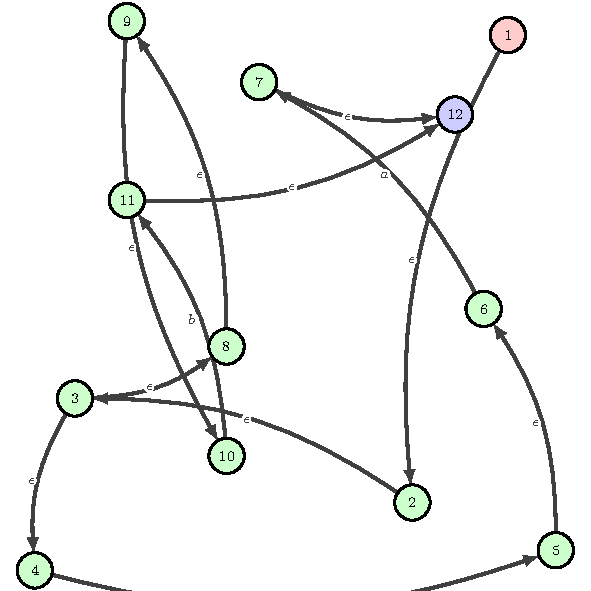
\includegraphics[width = 0.6\textwidth]{a|b}
  %\missingfigure{a|b}
  \caption{正则表达式$a|b$生成的NFA}
  \label{fig:ab}
\end{figure}

\cref{fig:ab}
中$6 \to 7$,$8 \to 11$展示了状态转换的逻辑,
但是算法中引入大量空串,
使生成$NFA$变得复杂,
对于像$(a|b)*ab$这样复杂的表达式()
视觉上很难识别转换关系
需要进一步化简。

% \cref{fig:complex}
\begin{figure}[H]
  \centering
  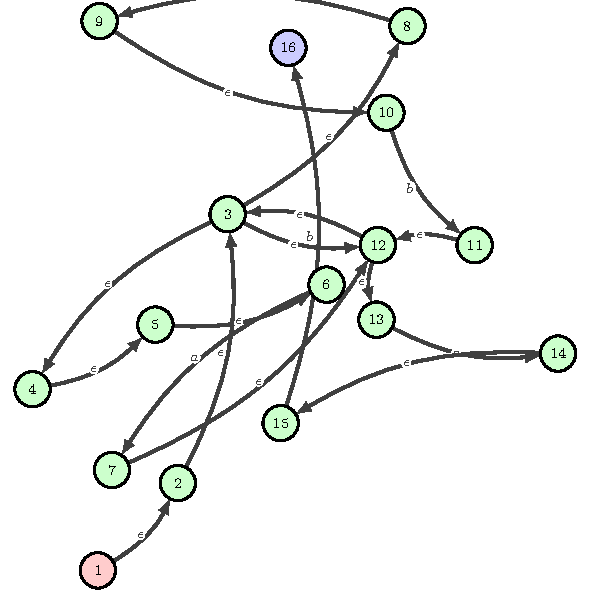
\includegraphics[width = 0.6\textwidth]{complex}
  %\missingfigure{complex}
  \caption{比较复杂的表达式$(a|b)*ab$}
  \label{fig:complex}
\end{figure}

\end{document}
